
%%%%%%%%%%%%%%%%%%%%%%%%%%%%%%%%%%%%%%%%%%%%%%%%%%%
\begin{frame}
  \begin{center}
    {\Large Sequences using PyTorch}
    
\tiny{(Ref:PyTorchZeroToAll  - Sung Kim )}
  \end{center}
\end{frame}



%%%%%%%%%%%%%%%%%%%%%%%%%%%%%%%%%%%%%%%%%%%%%%%%%%%
\begin{frame}[fragile] \frametitle{Recap (NN, CNN,RNN)}
\begin{center}
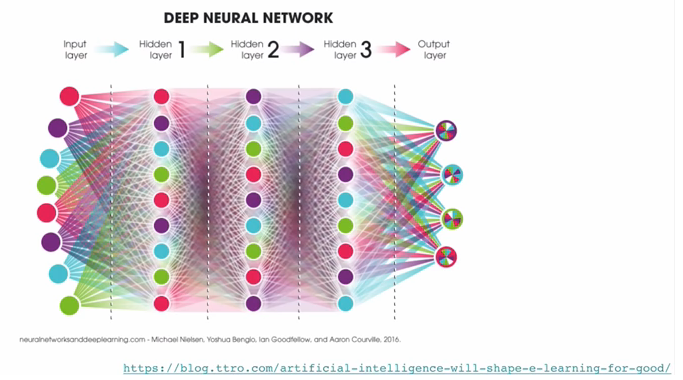
\includegraphics[width=0.8\linewidth,keepaspectratio]{pyrnn1}

\tiny{(Ref: PyTorch Lecture 12: RNN1 - Basics -Sung Kim)}
\end{center}
For given input, we fast forward to generate the output. Weights are adjusted during training so ast to match predicted and actual output as much as possible.
\end{frame}

%%%%%%%%%%%%%%%%%%%%%%%%%%%%%%%%%%%%%%%%%%%%%%%%%%%
\begin{frame}[fragile] \frametitle{Recap (NN, CNN,RNN)}
CNN
\begin{center}
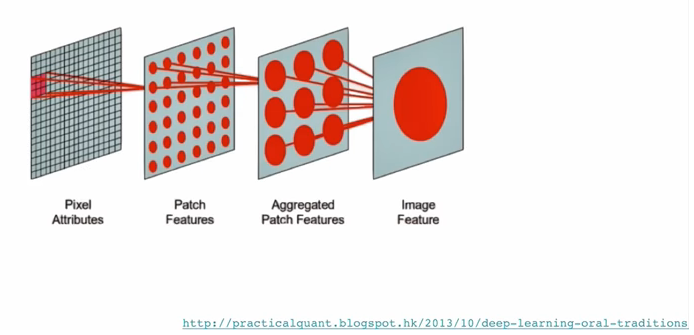
\includegraphics[width=0.8\linewidth,keepaspectratio]{pyrnn2}

\tiny{(Ref: PyTorch Lecture 12: RNN1 - Basics -Sung Kim)}
\end{center}
For given input, instead of using all of them together, we focus on certain areas, to extract features, then do similar thing in further layers. Finally you have NN to classify.
\end{frame}

%%%%%%%%%%%%%%%%%%%%%%%%%%%%%%%%%%%%%%%%%%%%%%%%%%%
\begin{frame}[fragile] \frametitle{Recap (NN, CNN,RNN)}
RNN
\begin{center}
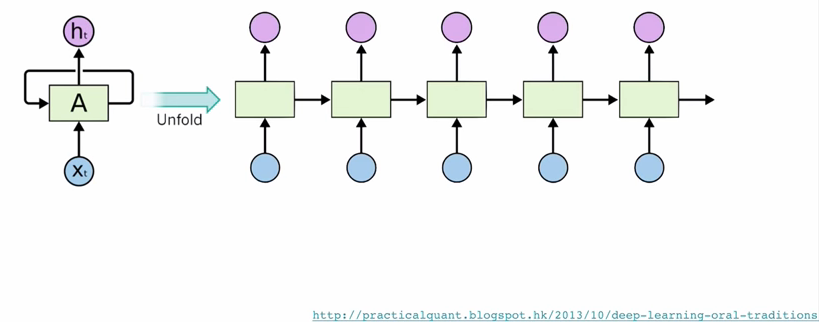
\includegraphics[width=0.8\linewidth,keepaspectratio]{pyrnn3}

\tiny{(Ref: PyTorch Lecture 12: RNN1 - Basics -Sung Kim)}
\end{center}
For given input, it produces output one by one. It also transfers hidden state to next time step to use for generating output along with input of that step.
Unfolded view means,each time step is shown differently, but actually its the same cell.
\end{frame}



%%%%%%%%%%%%%%%%%%%%%%%%%%%%%%%%%%%%%%%%%%%%%%%%%%%
\begin{frame}[fragile] \frametitle{LSTM in Pytorch}
\begin{itemize}
\item There are two styles of RNN modules. For example, nn.LSTM vs nn.LSTMcell. 
\item The former resembles the Torch7 counterpart, which works on a sequence. 
\item The latter only processes one element from the sequence at a time, so it can be completely replaced by the former one.
\end{itemize}

\end{frame}

%%%%%%%%%%%%%%%%%%%%%%%%%%%%%%%%%%%%%%%%%%%%%%%%%%%
\begin{frame}[fragile] \frametitle{LSTM in Pytorch}
\begin{itemize}
\item Input seq Variable has size [sequence\_length, batch\_size, input\_size].
\item More often than not, batch\_size is one.
\item Hidden state hc Variable is the initial hidden state.
\item num\_directions is 2 for bidirectional recurrent net.
\end{itemize}

\end{frame}

%%%%%%%%%%%%%%%%%%%%%%%%%%%%%%%%%%%%%%%%%%%%%%%%%%%
\begin{frame}[fragile] \frametitle{RNN}
\begin{center}
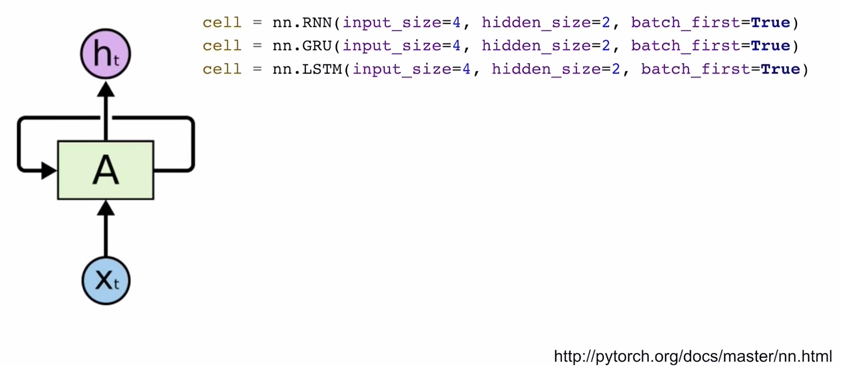
\includegraphics[width=\linewidth,keepaspectratio]{pyhun50}
\end{center}
Ready layer types are provided. ``hidden\_size'' is the output size.
\end{frame}

%%%%%%%%%%%%%%%%%%%%%%%%%%%%%%%%%%%%%%%%%%%%%%%%%%%
\begin{frame}[fragile] \frametitle{RNN}
\begin{center}
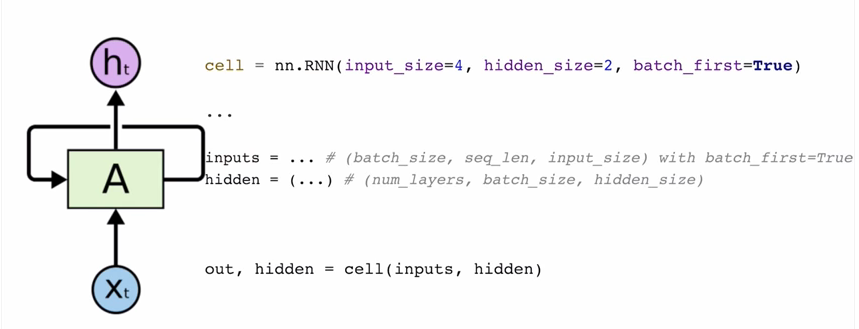
\includegraphics[width=\linewidth,keepaspectratio]{pyhun51}
\end{center}
\begin{itemize}
\item Each input has vector size 4 , so input\_size denotes word2vec dimension, eg \lstinline|'h' = [1,0,0,0]|
\item Output has vector size 2 , so hidden\_size denotes possible outcomes  eg \lstinline| = [x,x]|
\end{itemize}
\end{frame}

%%%%%%%%%%%%%%%%%%%%%%%%%%%%%%%%%%%%%%%%%%%%%%%%%%%
\begin{frame}[fragile] \frametitle{RNN}
\begin{center}
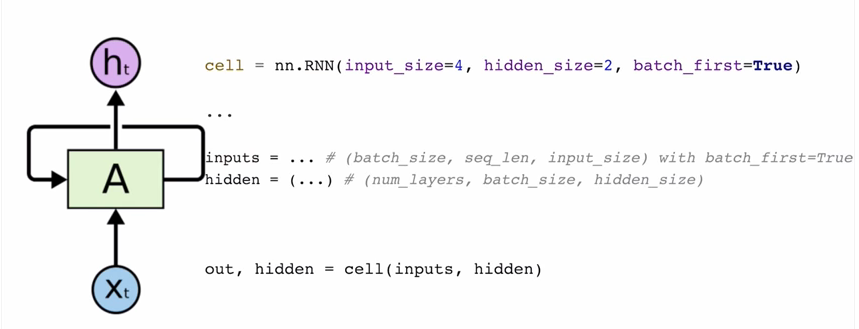
\includegraphics[width=\linewidth,keepaspectratio]{pyhun51}
\end{center}
\begin{itemize}
\item inputs are defined in terms of batch\_size, seq\_len, input\_size
\item  hidden states are defined in terms of num\_layers, batch\_size, hidden\_size
\end{itemize}
\end{frame}

%%%%%%%%%%%%%%%%%%%%%%%%%%%%%%%%%%%%%%%%%%%%%%%%%%%
\begin{frame}[fragile] \frametitle{RNN}
\begin{center}
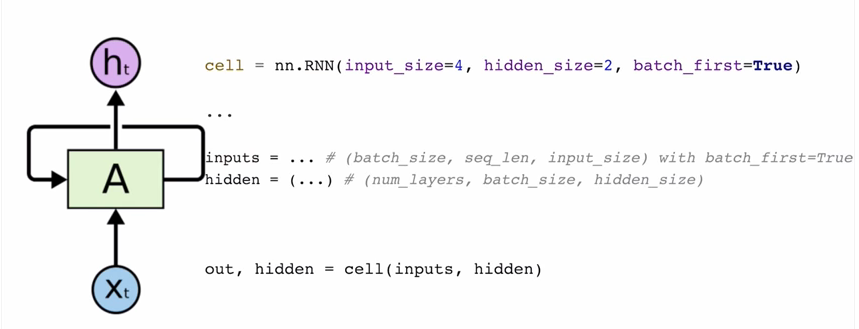
\includegraphics[width=\linewidth,keepaspectratio]{pyhun51}
\end{center}
\begin{itemize}
\item Generic way of using a `cell' has `out' and `hidden' as outputs.
\item The same `hidden' is passed as input in the next time step
\end{itemize}
\end{frame}

%%%%%%%%%%%%%%%%%%%%%%%%%%%%%%%%%%%%%%%%%%%%%%%%%%%
\begin{frame}[fragile] \frametitle{RNN: Example}
\begin{center}
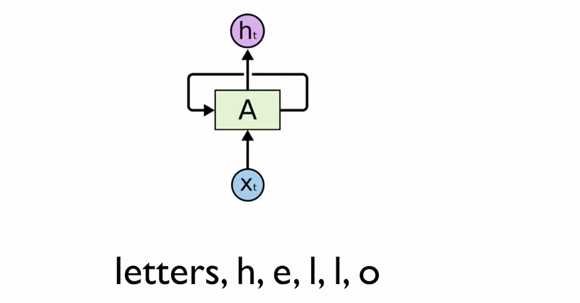
\includegraphics[width=0.6\linewidth,keepaspectratio]{pyrnn4}

\tiny{(Ref: PyTorch Lecture 12: RNN1 - Basics -Sung Kim)}
\end{center}
\begin{itemize}
\item Input: feed letters one by one. How to feed? Make each of them one hot encoded.
\item Output:two values are output-ed (?? for what??)
\end{itemize}
\end{frame}


%%%%%%%%%%%%%%%%%%%%%%%%%%%%%%%%%%%%%%%%%%%%%%%%%%%
\begin{frame}[fragile] \frametitle{RNN Input}

String ``hello'' is taken as one-hot encoded vectors. Input $x_t$ is vector instead of letter ``h''. Output $h_t$ is 2.
\begin{center}
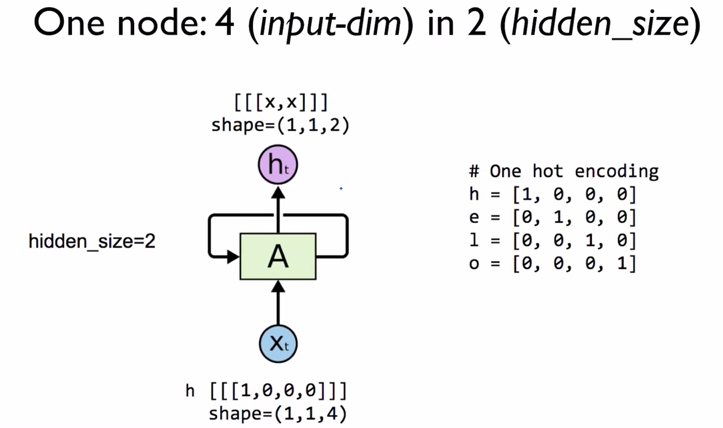
\includegraphics[width=0.8\linewidth,keepaspectratio]{pyhun52}
\end{center}
\end{frame}



%%%%%%%%%%%%%%%%%%%%%%%%%%%%%%%%%%%%%%%%%%%%%%%%%%%
\begin{frame}[fragile] \frametitle{RNN Input}
Code:
\begin{center}
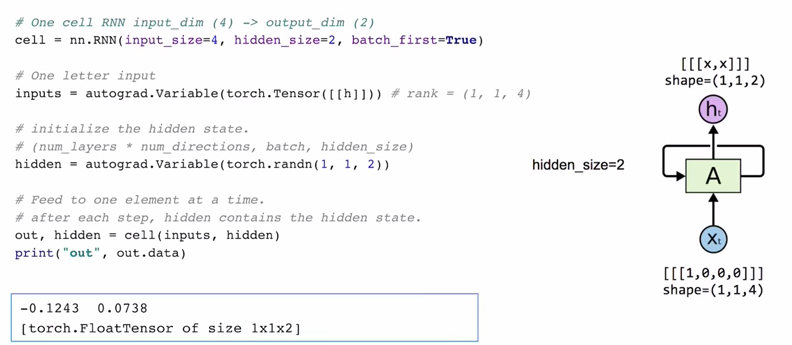
\includegraphics[width=0.8\linewidth,keepaspectratio]{pyhun53}
\end{center}

\begin{itemize}
\item First make a RNN cell by giving overall i/o sizes.
\item Dimensions of `inputs' is (1,1,4). First is batch size, second is number of words in a sentence and third is word2vec size.
\item Inputs being differentiable it is made as autograd Variable and initialized with one of the inputs `h'.
\end{itemize}
\end{frame}

%%%%%%%%%%%%%%%%%%%%%%%%%%%%%%%%%%%%%%%%%%%%%%%%%%%
\begin{frame}[fragile] \frametitle{RNN Input}
Code:
\begin{center}
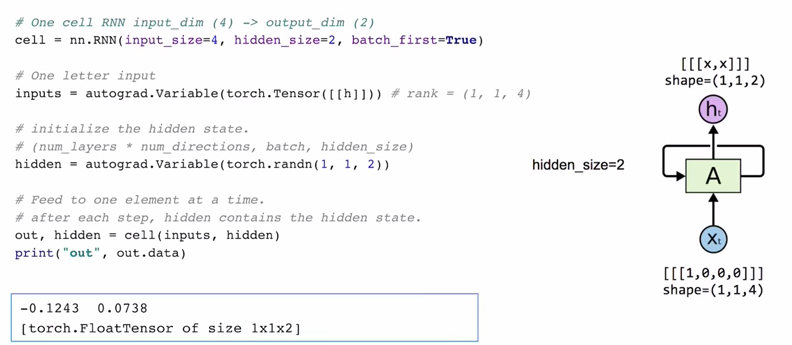
\includegraphics[width=0.8\linewidth,keepaspectratio]{pyhun53}
\end{center}

\begin{itemize}
\item Dimensions of `hidden' is (1,1,2). First is num layers * num directions , second is batch size and third is number of outcomes.
\item Hidden being differentiable it is made as autograd Variable. It it initialized with random values.
\end{itemize}
\end{frame}

%%%%%%%%%%%%%%%%%%%%%%%%%%%%%%%%%%%%%%%%%%%%%%%%%%%
\begin{frame}[fragile] \frametitle{RNN Input}

Putting 5 letters together as a sequence.

\begin{center}
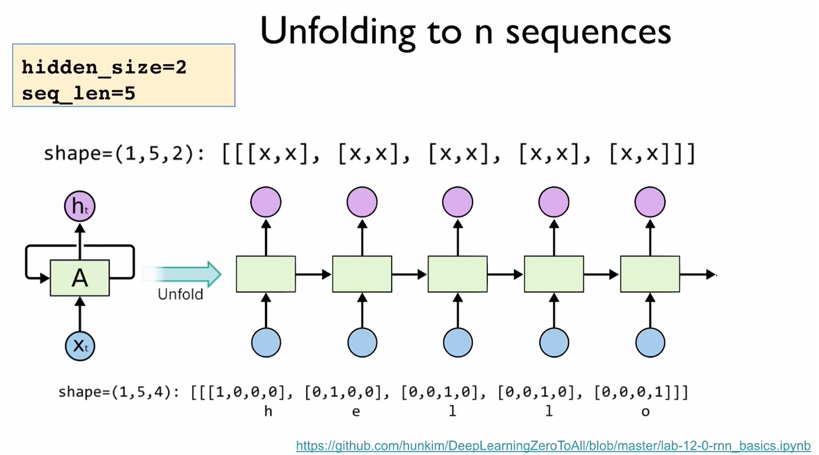
\includegraphics[width=0.8\linewidth,keepaspectratio]{pyhun54}
\end{center}

Input shape changes to (1,5,4) and output shape changes to (1,5,2)
\end{frame}

%%%%%%%%%%%%%%%%%%%%%%%%%%%%%%%%%%%%%%%%%%%%%%%%%%%
\begin{frame}[fragile] \frametitle{RNN Input}

\begin{center}
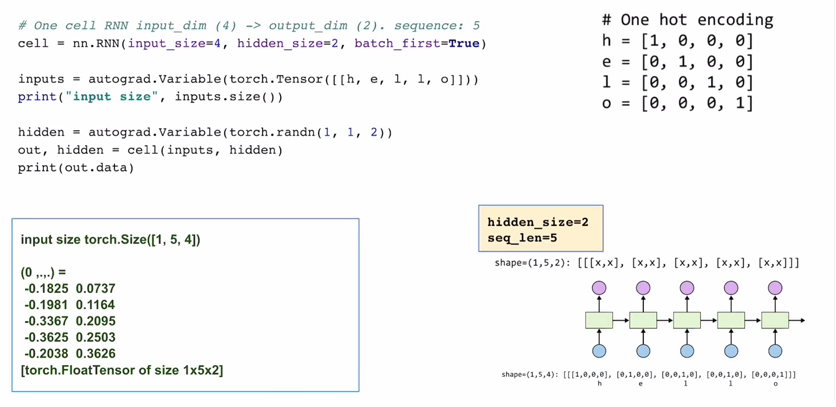
\includegraphics[width=0.8\linewidth,keepaspectratio]{pyrnn5}

\tiny{(Ref: PyTorch Lecture 12: RNN1 - Basics -Sung Kim)}
\end{center}
\begin{itemize}
\item See how inputs Variable has been initialized with a sequence.
\item Output is now set of 5 pairs, one for each input character.
\end{itemize}
\end{frame}


%%%%%%%%%%%%%%%%%%%%%%%%%%%%%%%%%%%%%%%%%%%%%%%%%%%
\begin{frame}[fragile] \frametitle{RNN Input}

Want to break input into 3 batches.

\begin{center}
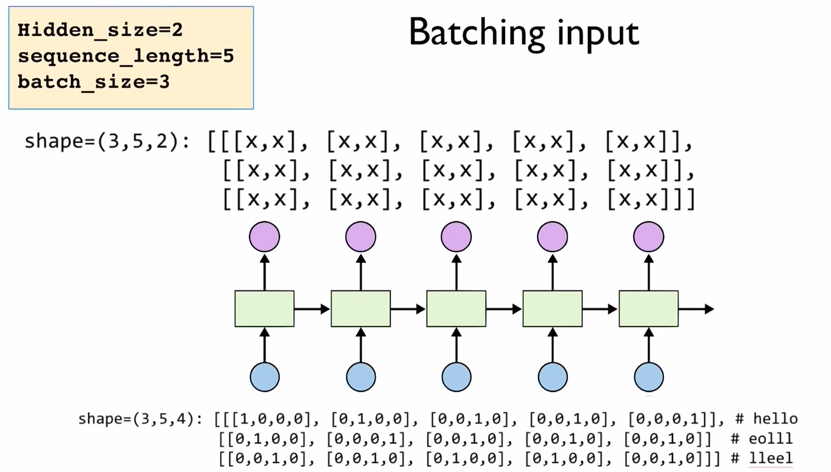
\includegraphics[width=0.8\linewidth,keepaspectratio]{pyhun55}
\end{center}
Input shape changes to (3,5,4) and output shape changes to (3,5,2)
\end{frame}

%%%%%%%%%%%%%%%%%%%%%%%%%%%%%%%%%%%%%%%%%%%%%%%%%%%
\begin{frame}[fragile] \frametitle{RNN Input}

\begin{center}
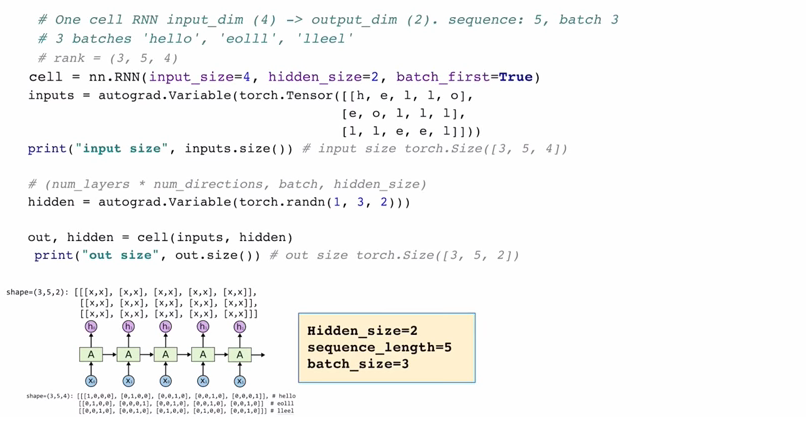
\includegraphics[width=0.8\linewidth,keepaspectratio]{pyrnn6}
\end{center}
\begin{itemize}
\item See how a batch of 3 sequences are passed with 5 inputs each, each having 4 dim word2vec.
\item Correspondingly hidden also has batch size same as inputs.
\end{itemize}
\end{frame}

%%%%%%%%%%%%%%%%%%%%%%%%%%%%%%%%%%%%%%%%%%%%%%%%%%%
\begin{frame}[fragile] \frametitle{Summary regarding dimensions}


\begin{itemize}
\item Batch size is number of sequences or sentences at a time (no weights update while a batch is running)
\item Sequence length: number of words in a sequence/sentence.
\item Input size is the dimension of vector representation of a word. In case of One Hot Encoding, it becomes Vocab size.
\item Hidden size which is same as Output size is the number of outcomes you need.
\item Num Layers can be decided as per need, same as num directions (1 for uni, 2 for bi directional)
\end{itemize}
\end{frame}




%%%%%%%%%%%%%%%%%%%%%%%%%%%%%%%%%%%%%%%%%%%%%%%%%%%
\begin{frame}[fragile] \frametitle{RNN Input}

Language modeling: predicting next character.

\begin{center}
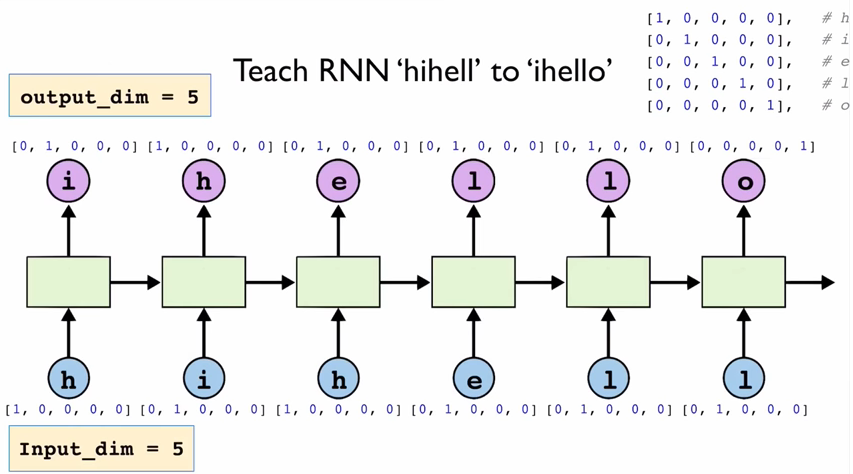
\includegraphics[width=0.8\linewidth,keepaspectratio]{pyhun56}

\tiny{(Ref: PyTorch Lecture 12: RNN1 - Basics -Sung Kim)}
\end{center}
Both, input and output dimensions are 5. Multi class classification.
\end{frame}

%%%%%%%%%%%%%%%%%%%%%%%%%%%%%%%%%%%%%%%%%%%%%%%%%%%
\begin{frame}[fragile] \frametitle{RNN Loss and Training}

\begin{center}
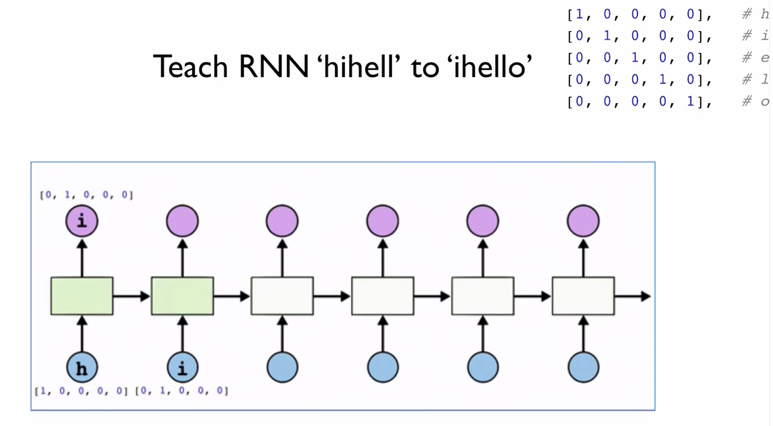
\includegraphics[width=0.8\linewidth,keepaspectratio]{pyrnn7}

\tiny{(Ref: PyTorch Lecture 12: RNN1 - Basics -Sung Kim)}
\end{center}
One word at a time is fed in. It is trained against known next letter.
\end{frame}

%%%%%%%%%%%%%%%%%%%%%%%%%%%%%%%%%%%%%%%%%%%%%%%%%%%
\begin{frame}[fragile] \frametitle{RNN Loss and Training}

Language modeling: predicting next character.

\begin{center}
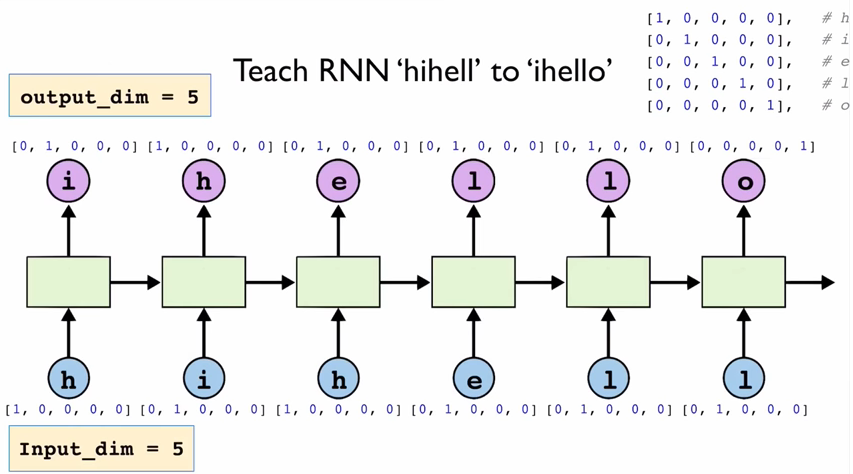
\includegraphics[width=0.8\linewidth,keepaspectratio]{pyhun56}

\tiny{(Ref: PyTorch Lecture 12: RNN1 - Basics -Sung Kim)}
\end{center}
Both, input and output dimensions are 5. 
\end{frame}

%%%%%%%%%%%%%%%%%%%%%%%%%%%%%%%%%%%%%%%%%%%%%%%%%%%
\begin{frame}[fragile] \frametitle{RNN Loss and Training}

\begin{center}
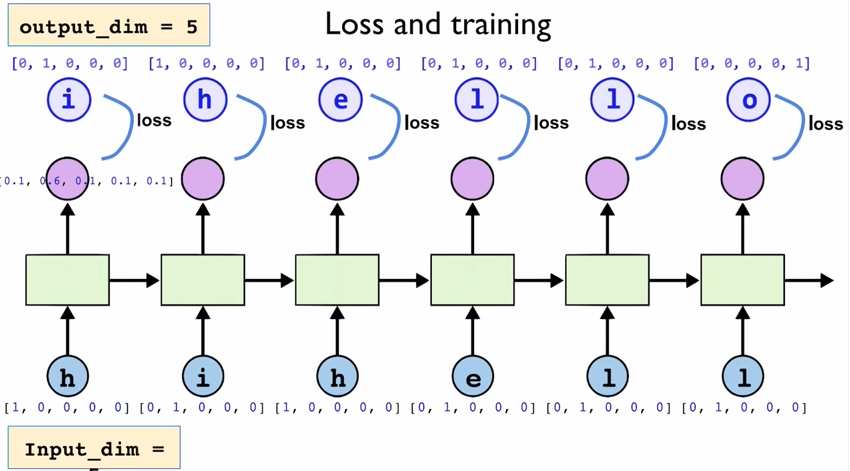
\includegraphics[width=0.8\linewidth,keepaspectratio]{pyhun57}

\tiny{(Ref: PyTorch Lecture 12: RNN1 - Basics -Sung Kim)}
\end{center}

Diff is there in predicted and the actual(next) letter. As its Multi Class problem the loss is by Cross Entropy. Its applied to each node and the loss is summed.
\end{frame}


%%%%%%%%%%%%%%%%%%%%%%%%%%%%%%%%%%%%%%%%%%%%%%%%%%%
\begin{frame}[fragile] \frametitle{RNN Data Preparation}

\begin{center}
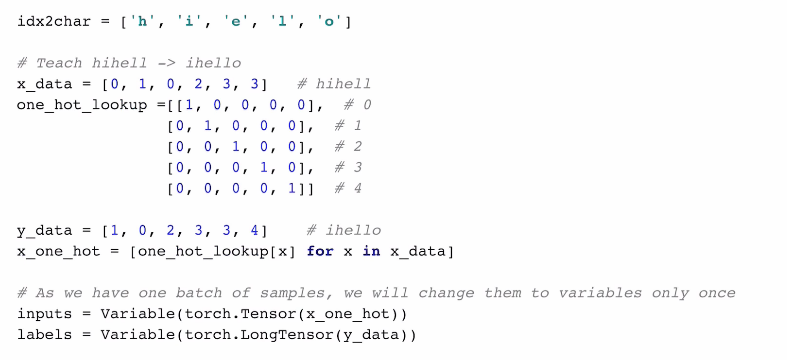
\includegraphics[width=\linewidth,keepaspectratio]{pyhun58}

\tiny{(Ref: PyTorch Lecture 12: RNN1 - Basics -Sung Kim)}
\end{center}

First make index of characters. So `h' is 0 , `i' is 1 and so on. Make `x' which is `hihell' in terms of index ids. Then make a character to one-hot dictionary. Use it convert from `x' to `x\_one\_hot', but keep y labels only in index ids (for `ihello') and not in one-hot equivalents.
\end{frame}


%%%%%%%%%%%%%%%%%%%%%%%%%%%%%%%%%%%%%%%%%%%%%%%%%%%
\begin{frame}[fragile] \frametitle{RNN Parameters}

\begin{center}
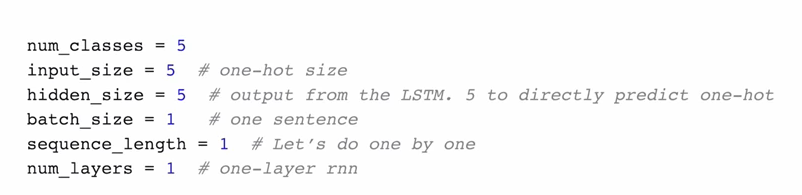
\includegraphics[width=\linewidth,keepaspectratio]{pyrnn8}

\tiny{(Ref: PyTorch Lecture 12: RNN1 - Basics -Sung Kim)}
\end{center}

\begin{itemize}
\item Number of classes: how many output values you need to predict at a time, for one hot of a output word, we need 5.
\item Input is one hot size or the vocab size
\item Output size is same as output size
\item Sequence length is number of words in a sentence , its set to 1, so only one word at a time
\item Num layers have been kept at minimum 1.
\end{itemize}
\end{frame}


%%%%%%%%%%%%%%%%%%%%%%%%%%%%%%%%%%%%%%%%%%%%%%%%%%%
\begin{frame}[fragile] \frametitle{RNN Parameters}

\begin{center}
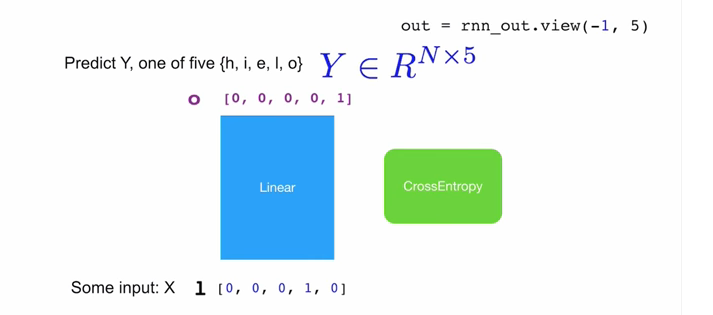
\includegraphics[width=\linewidth,keepaspectratio]{pyrnn9}

\tiny{(Ref: PyTorch Lecture 12: RNN1 - Basics -Sung Kim)}
\end{center}

\begin{itemize}
\item Output size is 5 being size of the one hot encoding. But how many such woulds would be out?
\item It would be variable `N', an unknown, so kept as $-1$.
\end{itemize}
\end{frame}



%%%%%%%%%%%%%%%%%%%%%%%%%%%%%%%%%%%%%%%%%%%%%%%%%%%
\begin{frame}[fragile] \frametitle{RNN Model}

\begin{center}
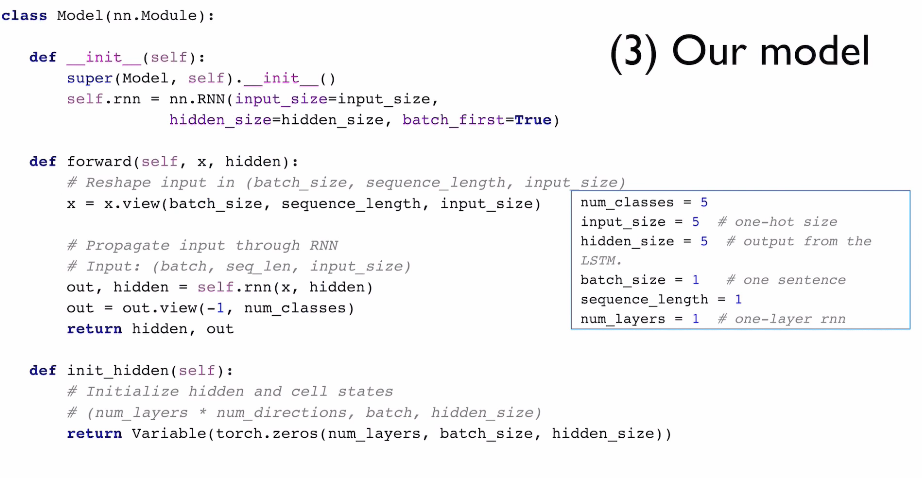
\includegraphics[width=\linewidth,keepaspectratio]{pyhun59}

\tiny{(Ref: PyTorch Lecture 12: RNN1 - Basics -Sung Kim)}
\end{center}

Parameters are set properly and reused in definition of model.
\end{frame}


%%%%%%%%%%%%%%%%%%%%%%%%%%%%%%%%%%%%%%%%%%%%%%%%%%%
\begin{frame}[fragile] \frametitle{RNN Training}

\begin{center}
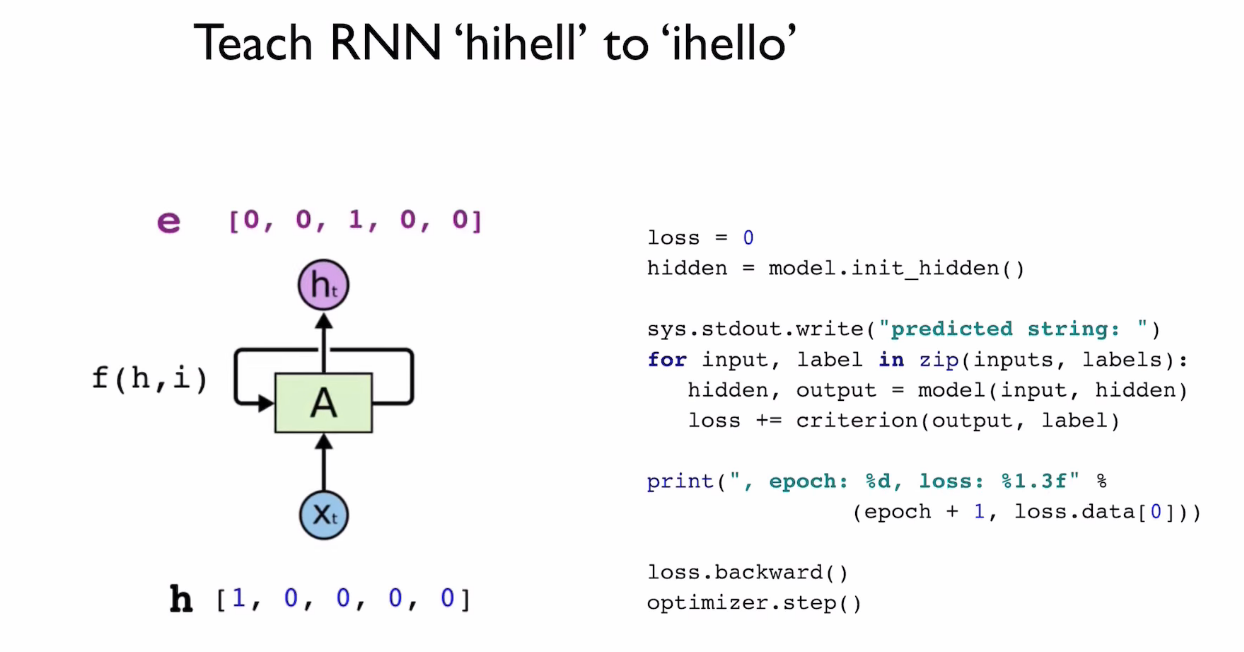
\includegraphics[width=\linewidth,keepaspectratio]{pyhun60}

\tiny{(Ref: PyTorch Lecture 12: RNN1 - Basics -Sung Kim)}
\end{center}


\end{frame}


%%%%%%%%%%%%%%%%%%%%%%%%%%%%%%%%%%%%%%%%%%%%%%%%%%%
\begin{frame}[fragile] \frametitle{RNN Results}

\begin{center}
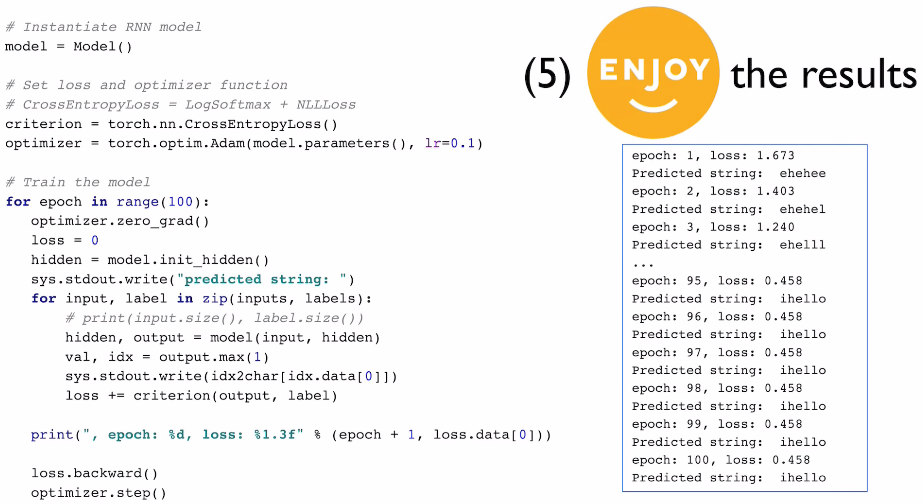
\includegraphics[width=\linewidth,keepaspectratio]{pyhun61}

\tiny{(Ref: PyTorch Lecture 12: RNN1 - Basics -Sung Kim)}
\end{center}


\end{frame}

%%%%%%%%%%%%%%%%%%%%%%%%%%%%%%%%%%%%%%%%%%%%%%%%%%%
\begin{frame}[fragile] \frametitle{RNN Training}

\begin{center}
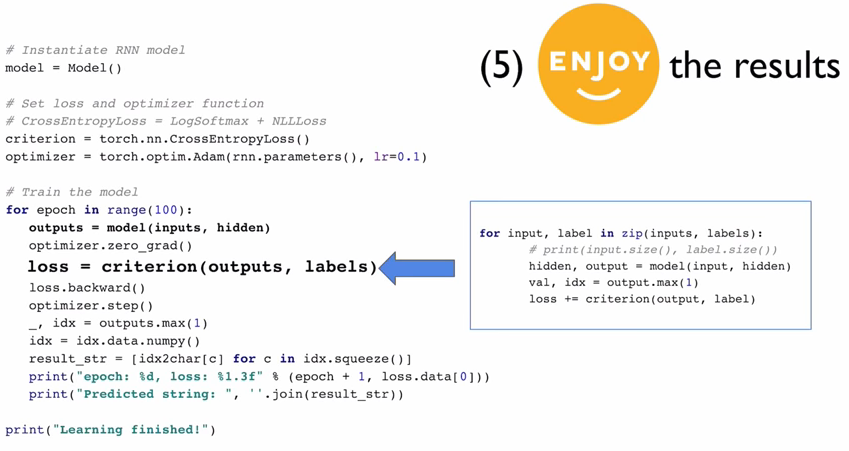
\includegraphics[width=0.8\linewidth,keepaspectratio]{pyrnn10}

\tiny{(Ref: PyTorch Lecture 12: RNN1 - Basics -Sung Kim)}
\end{center}

\begin{itemize}
\item Instead of feeding one character at a time in a for loop, you can supply whole input array at ones. And also corresponding labels array at the same time.
\item In each epoch, weights get refined for same pair of inputs and labels.
\item Make sure you zero the grads at before back propagation.
\end{itemize}
\end{frame}

%%%%%%%%%%%%%%%%%%%%%%%%%%%%%%%%%%%%%%%%%%%%%%%%%%%
\begin{frame}[fragile] \frametitle{If NN instead of RNN}

\begin{center}
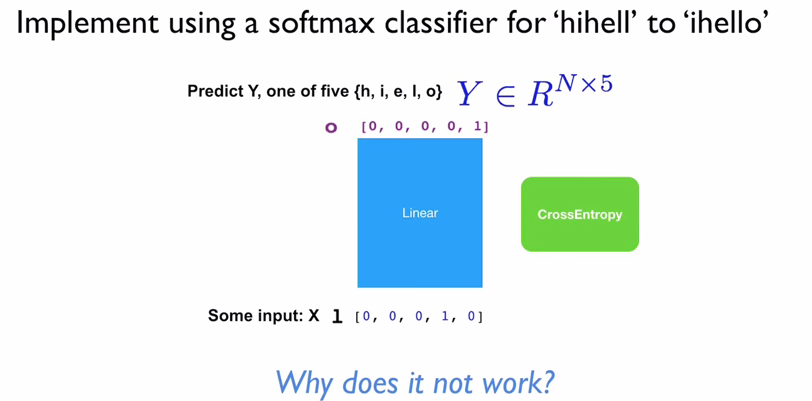
\includegraphics[width=0.8\linewidth,keepaspectratio]{pyrnn11}

\tiny{(Ref: PyTorch Lecture 12: RNN1 - Basics -Sung Kim)}
\end{center}

\begin{itemize}
\item If we had used simple NN (ie softmax multi class classifier) the results would not be good.
\item It does not take into account the previous inputs, but just one independent input at a time.
\end{itemize}
\end{frame}

%%%%%%%%%%%%%%%%%%%%%%%%%%%%%%%%%%%%%%%%%%%%%%%%%%%
\begin{frame}[fragile] \frametitle{RNN +  NN}

\begin{center}
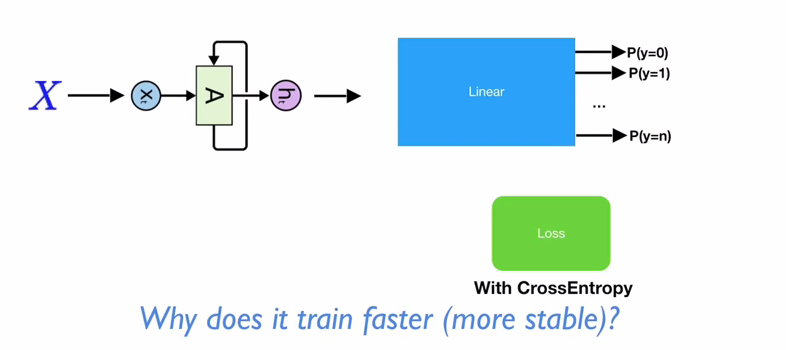
\includegraphics[width=0.8\linewidth,keepaspectratio]{pyrnn12}

\tiny{(Ref: PyTorch Lecture 12: RNN1 - Basics -Sung Kim)}
\end{center}

\begin{itemize}
\item Output of RNN is fed into normal NN (softmax)
\item So both RNN and NN weights would get refined during training.
\end{itemize}
\end{frame}


%%%%%%%%%%%%%%%%%%%%%%%%%%%%%%%%%%%%%%%%%%%%%%%%%%%
\begin{frame}[fragile] \frametitle{Word2Vec in place of One Hot}

\begin{center}
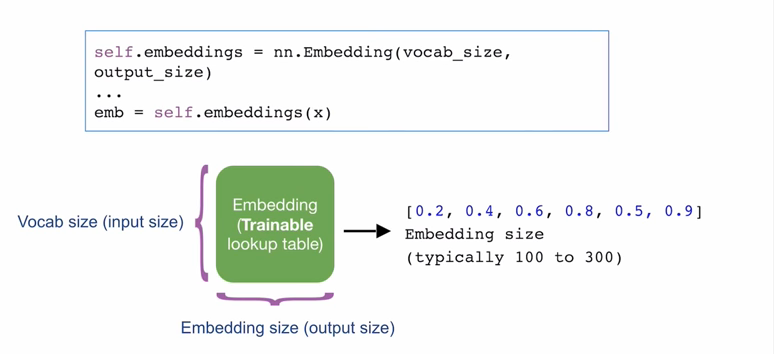
\includegraphics[width=0.8\linewidth,keepaspectratio]{pyrnn13}

\tiny{(Ref: PyTorch Lecture 12: RNN1 - Basics -Sung Kim)}
\end{center}

\begin{itemize}
\item Pytorch give word2vec generator by itself.
\item Need to supply vocab size and output dimension size (say 100, 300)
\item Passing x, a word to vec generator/lookup is prepared.
\end{itemize}
\end{frame}


%%%%%%%%%%%%%%%%%%%%%%%%%%%%%%%%%%%%%%%%%%%%%%%%%%%
\begin{frame}[fragile] \frametitle{RNN: Under the hood (Recap)}

\begin{center}
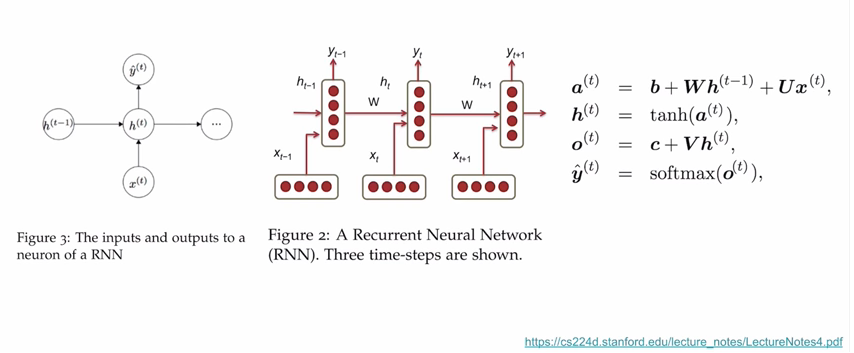
\includegraphics[width=\linewidth,keepaspectratio]{pyrnn14}

\tiny{(Ref: PyTorch Lecture 12: RNN1 - Basics -Sung Kim)}
\end{center}
Weights like $W,U,V$ and biases $b,c$ are refined in training.
\end{frame}

%%%%%%%%%%%%%%%%%%%%%%%%%%%%%%%%%%%%%%%%%%%%%%%%%%%
\begin{frame}
  \begin{center}
    {\Large RNN For Classification}
    
\tiny{(Ref:  PyTorch Lecture 13: RNN2 - Classification -Sung Kim )}
  \end{center}
\end{frame}



%%%%%%%%%%%%%%%%%%%%%%%%%%%%%%%%%%%%%%%%%%%%%%%%%%%
\begin{frame}[fragile] \frametitle{RNN For Classification}

\begin{itemize}
\item Input: Name (characters)
\item Output: Country Name (Enum, 18 categories)
\end{itemize}

 
 
\begin{center}
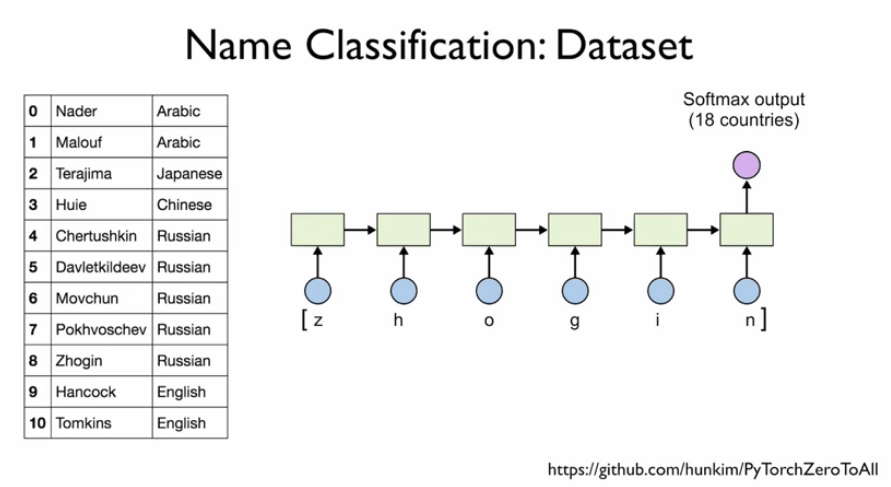
\includegraphics[width=0.8\linewidth,keepaspectratio]{pyhun65}

\tiny{(Ref:  PyTorch Lecture 13: RNN2 - Classification -Sung Kim )}
\end{center}


\end{frame}

%%%%%%%%%%%%%%%%%%%%%%%%%%%%%%%%%%%%%%%%%%%%%%%%%%%
\begin{frame}[fragile] \frametitle{RNN For Classification}

 
\begin{center}
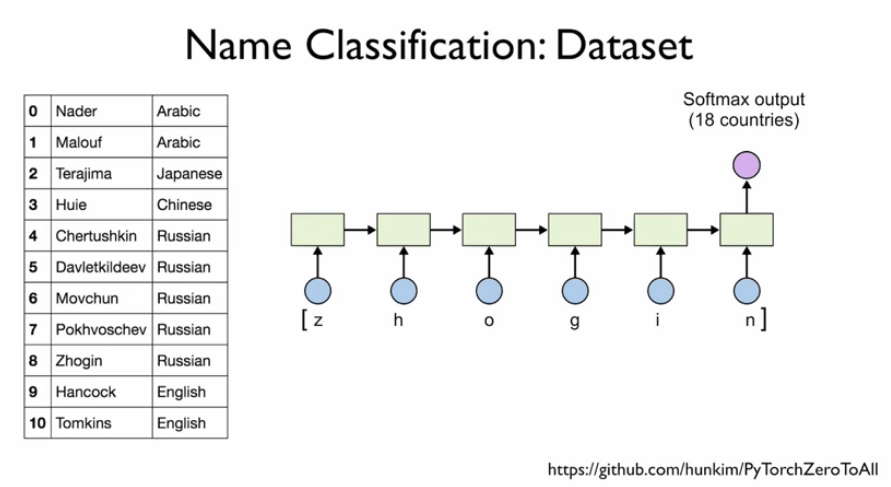
\includegraphics[width=0.8\linewidth,keepaspectratio]{pyhun65}

\tiny{(Ref:  PyTorch Lecture 13: RNN2 - Classification -Sung Kim )}
\end{center}
\begin{itemize}
\item As shown, for a name `Zhogin', characters are fed one by one, in each time step.
\item Hidden states are passed, and only at the end, only one output value (softmax-ed) is generated.
\end{itemize}

\end{frame}

%%%%%%%%%%%%%%%%%%%%%%%%%%%%%%%%%%%%%%%%%%%%%%%%%%%
\begin{frame}[fragile] \frametitle{Preparing Input}

 
\begin{center}
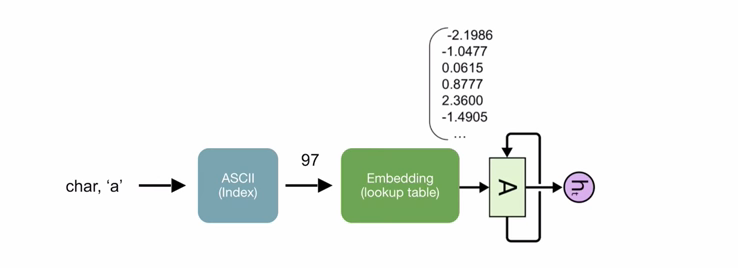
\includegraphics[width=0.8\linewidth,keepaspectratio]{pyrnn15}

\tiny{(Ref:  PyTorch Lecture 13: RNN2 - Classification -Sung Kim )}
\end{center}
\begin{itemize}
\item Each character is converted to id (simplest way is to get its ASCII number)
\item Then pass through embedding look up which is made by whole vocab of characters. It a table of id (ASCII) vs word2vec
\item Embeddings are trained based on vocab
\end{itemize}

\end{frame}

%%%%%%%%%%%%%%%%%%%%%%%%%%%%%%%%%%%%%%%%%%%%%%%%%%%
\begin{frame}[fragile] \frametitle{Preparing Input}

\begin{center}
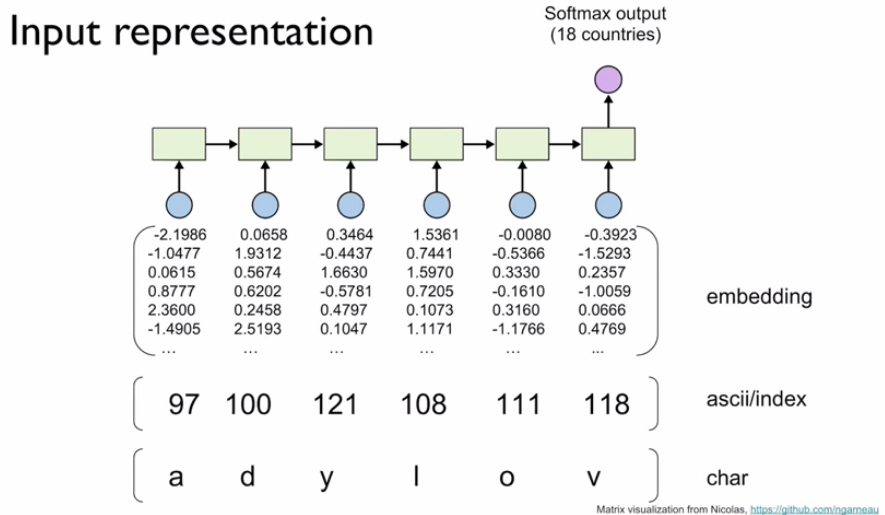
\includegraphics[width=0.8\linewidth,keepaspectratio]{pyhun62}

\tiny{(Ref:  PyTorch Lecture 13: RNN2 - Classification -Sung Kim )}
\end{center}


\end{frame}

%%%%%%%%%%%%%%%%%%%%%%%%%%%%%%%%%%%%%%%%%%%%%%%%%%%
\begin{frame}[fragile] \frametitle{RNN For Classification}

\begin{center}
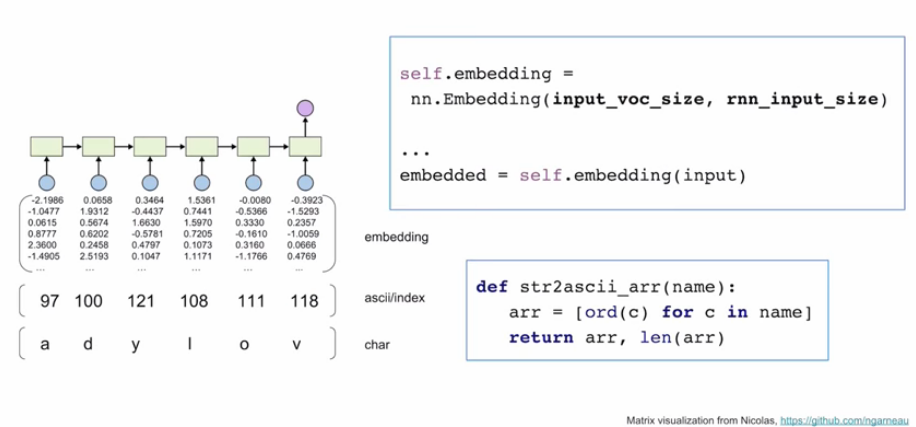
\includegraphics[width=\linewidth,keepaspectratio]{pyhun63}

\tiny{(Ref:  PyTorch Lecture 13: RNN2 - Classification -Sung Kim )}
\end{center}

\begin{itemize}
\item Ord returns ASCII code to a character. 
\item Embedding layer is Word2Vec like vectors.
\item input\_voc\_size is size of all ASCII indices.
\item rnn\_input\_size is the word2vec size, may be 300
\end{itemize}
\end{frame}


%%%%%%%%%%%%%%%%%%%%%%%%%%%%%%%%%%%%%%%%%%%%%%%%%%%
\begin{frame}[fragile] \frametitle{RNN For Classification Code}
\begin{center}
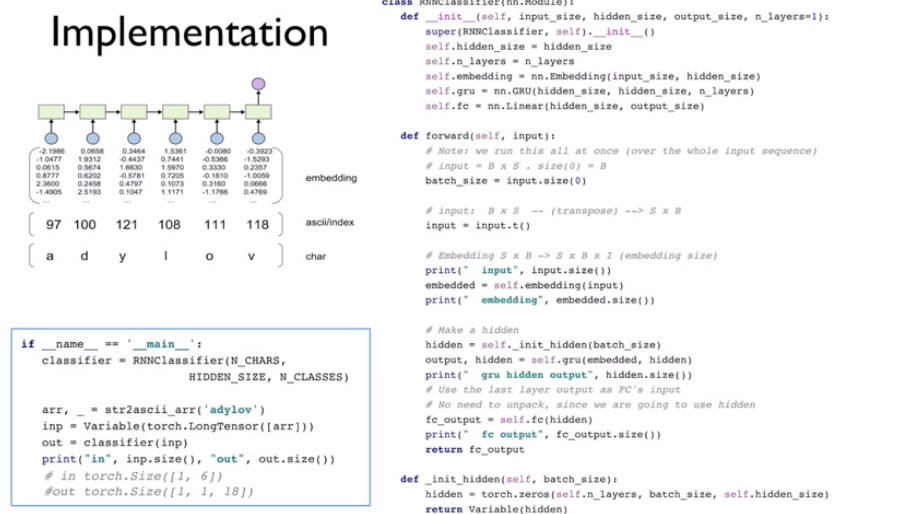
\includegraphics[width=\linewidth,keepaspectratio]{pyhun64}
\end{center}
\end{frame}

%%%%%%%%%%%%%%%%%%%%%%%%%%%%%%%%%%%%%%%%%%%%%%%%%%%
\begin{frame}[fragile] \frametitle{RNN For Classification Code}
\begin{center}
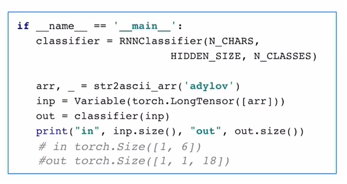
\includegraphics[width=0.4\linewidth,keepaspectratio]{pyrnn17}
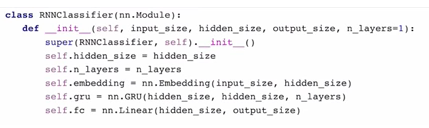
\includegraphics[width=0.55\linewidth,keepaspectratio]{pyrnn18}
\end{center}
\begin{itemize}
\item Actual testing/usage is shown in box (in Pytorch there seems no separate feeding inputs and fitting/training and predicting. Right from first input, with initial random weights, it starts predicting output.
\item If you run this through epochs,comparing with actual, back-propagating on loss, the output would be refined.
\end{itemize}

\end{frame}

%%%%%%%%%%%%%%%%%%%%%%%%%%%%%%%%%%%%%%%%%%%%%%%%%%%
\begin{frame}[fragile] \frametitle{RNN For Classification Code}
\begin{center}
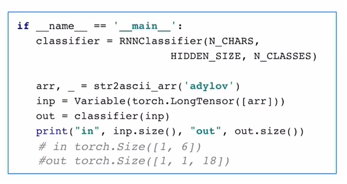
\includegraphics[width=0.4\linewidth,keepaspectratio]{pyrnn17}
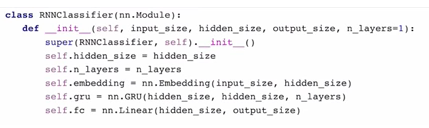
\includegraphics[width=0.55\linewidth,keepaspectratio]{pyrnn18}
\end{center}
\begin{itemize}
\item input\_size :same as vocab of ASCII, set to N\_CHARS = 128
\item hidden\_size:  word2vec length for embeddings layer, set to HIDDEN\_SIZE= 100
\item output\_size : number of outcomes, 18 counties in this case, set to N\_CLASSES = 18
\end{itemize}

\end{frame}

%%%%%%%%%%%%%%%%%%%%%%%%%%%%%%%%%%%%%%%%%%%%%%%%%%%
\begin{frame}[fragile] \frametitle{RNN For Classification Code}
\begin{center}
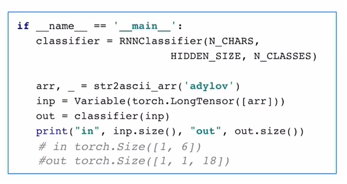
\includegraphics[width=0.4\linewidth,keepaspectratio]{pyrnn17}
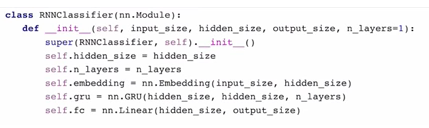
\includegraphics[width=0.55\linewidth,keepaspectratio]{pyrnn18}
\end{center}
\begin{itemize}
\item In init() we populate 3 sub networks : embedding, GRU and Linear
\item For embedding, input size is vocab length 128, output is embedding length 100
\item For GRU, input and output size are both same, ie given by hidden size, ie word2vec dimension, ie embedding size, 100.
\item For Linear, ie fully connected dense NN, input is embedding size 100, output is 18 classes. It has softmax at the end.
\end{itemize}

\end{frame}

%%%%%%%%%%%%%%%%%%%%%%%%%%%%%%%%%%%%%%%%%%%%%%%%%%%
\begin{frame}[fragile] \frametitle{RNN For Classification Code}
\begin{center}
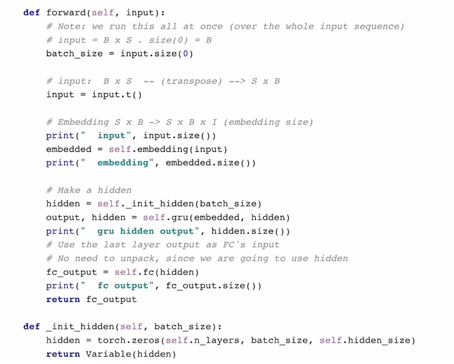
\includegraphics[width=0.55\linewidth,keepaspectratio]{pyrnn19}
\end{center}
\begin{itemize}
\item forward() gets called when model(x) is called.
\item Its code says, how input processed into output. 
\item It connects layers in right order for right input. 
\item Shape (Batch Size x Input Size) ie $B=1 \times S=6$ characters
\end{itemize}

\end{frame}


%%%%%%%%%%%%%%%%%%%%%%%%%%%%%%%%%%%%%%%%%%%%%%%%%%%
\begin{frame}[fragile] \frametitle{RNN For Classification Code}
\begin{center}
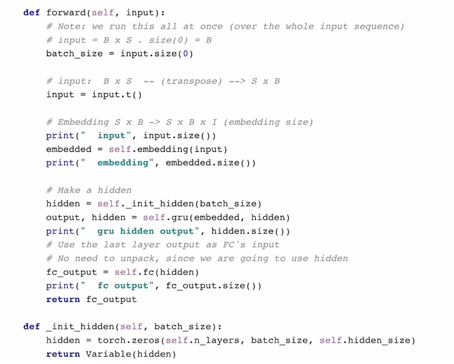
\includegraphics[width=0.55\linewidth,keepaspectratio]{pyrnn19}
\end{center}
\begin{itemize}
\item Embedding converts $S \times B \rightarrow S \times B \times I $
\item 3D array with 6 x 1 x 100 dims
\item This goes as input to GRU layer
\end{itemize}
\end{frame}


%%%%%%%%%%%%%%%%%%%%%%%%%%%%%%%%%%%%%%%%%%%%%%%%%%%
\begin{frame}[fragile] \frametitle{RNN For Classification Code}
\begin{center}
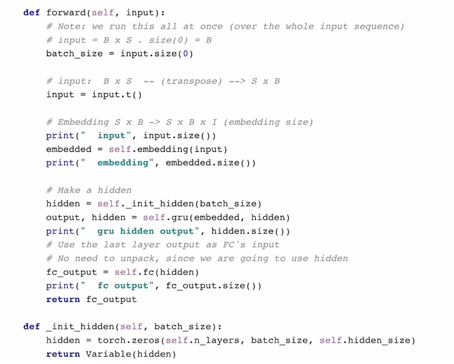
\includegraphics[width=0.55\linewidth,keepaspectratio]{pyrnn19}
\end{center}
\begin{itemize}
\item We initialize the `hidden' with a custom function (zeros).
\item Thats passed as input to GRU, which in turn generates `output' as well as next/last timestep `hidden'.
\item `output' is forgotten, and the `hidden' is passed to Linear layer. 

\end{itemize}
\end{frame}

%%%%%%%%%%%%%%%%%%%%%%%%%%%%%%%%%%%%%%%%%%%%%%%%%%%
\begin{frame}[fragile] \frametitle{RNN For Classification Code}
\begin{center}
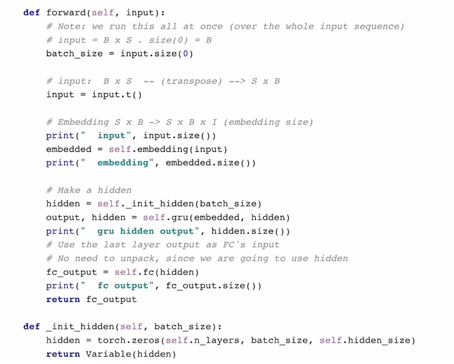
\includegraphics[width=0.55\linewidth,keepaspectratio]{pyrnn19}
\end{center}
\begin{itemize}
\item In the digram we saw that `hidden' is used and not the `output'. But it can also be used.
\item NN predicts the final outcome. Note that this then needs to be checked with actual, then calculate loss, and backprop to optimize.
\end{itemize}
\end{frame}

%%%%%%%%%%%%%%%%%%%%%%%%%%%%%%%%%%%%%%%%%%%%%%%%%%%
\begin{frame}[fragile] \frametitle{RNN For Classification Code}
\begin{center}
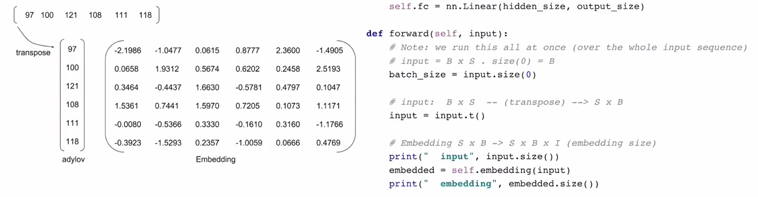
\includegraphics[width=\linewidth,keepaspectratio]{pyrnn20}
\end{center}
\begin{itemize}
\item Note that the Transpose operation should not be forgotten.
\item Initial input is just ASCII indices of each character in the word `adylov' (1 x 6)
\item Transpose makes it vertical column each row as a character. (6 x 1)
\item Embedding shown is the output of this layer.
\end{itemize}
\end{frame}



%%%%%%%%%%%%%%%%%%%%%%%%%%%%%%%%%%%%%%%%%%%%%%%%%%%
\begin{frame}[fragile] \frametitle{Batches}
\begin{itemize}
\item But we want to look at many names with different lengths. 
\item Just using for loop is not sufficient, we want to get it in a single uniform structure.
\item Variable length input in a batch.
\item In a batch all have to be of same length.
\item Its done by padding.
\item Then whole batch is converted to embedded vectors.
\end{itemize}
\end{frame}


%%%%%%%%%%%%%%%%%%%%%%%%%%%%%%%%%%%%%%%%%%%%%%%%%%%
\begin{frame}[fragile] \frametitle{Batches}
\begin{center}
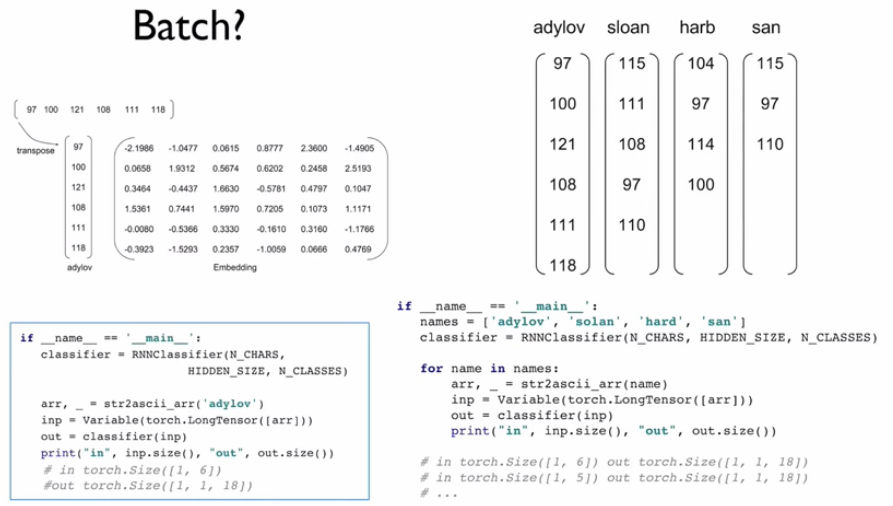
\includegraphics[width=0.8\linewidth,keepaspectratio]{pyhun66}
\end{center}
\end{frame}

%%%%%%%%%%%%%%%%%%%%%%%%%%%%%%%%%%%%%%%%%%%%%%%%%%%
\begin{frame}[fragile] \frametitle{Padding}
``0'' marks end of the string.

\begin{center}
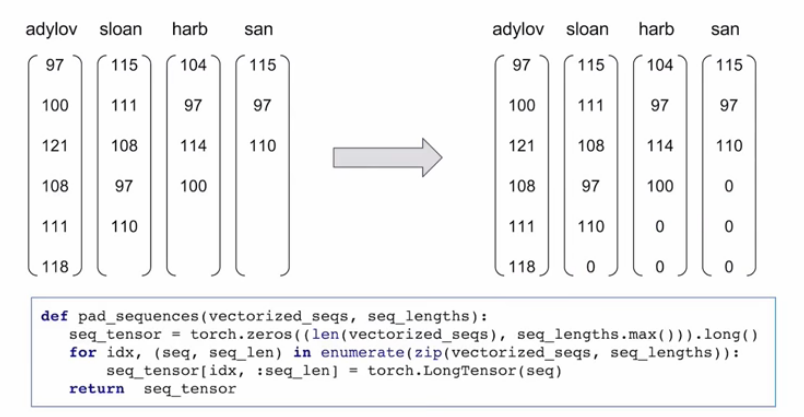
\includegraphics[width=\linewidth,keepaspectratio]{pyhun67}
\end{center}
\end{frame}

%%%%%%%%%%%%%%%%%%%%%%%%%%%%%%%%%%%%%%%%%%%%%%%%%%%
\begin{frame}[fragile] \frametitle{Embedding}
\begin{center}
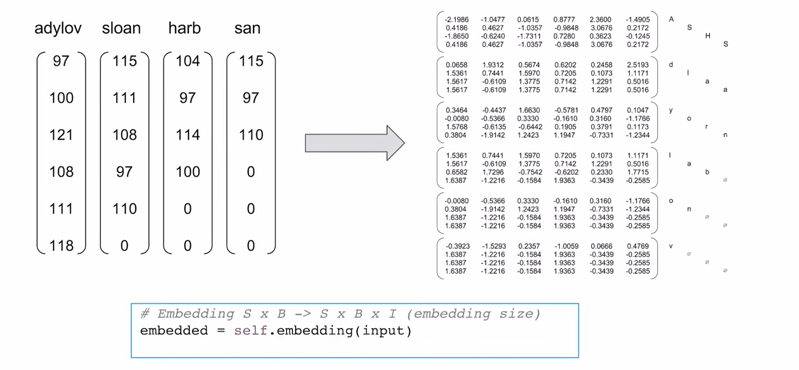
\includegraphics[width=\linewidth,keepaspectratio]{pyrnn21}
\end{center}
\end{frame}



%%%%%%%%%%%%%%%%%%%%%%%%%%%%%%%%%%%%%%%%%%%%%%%%%%%
\begin{frame}[fragile] \frametitle{Full Implementation}
\begin{center}
\includegraphics[width=\linewidth,keepaspectratio]{pyhun68}
\end{center}
\end{frame}

%%%%%%%%%%%%%%%%%%%%%%%%%%%%%%%%%%%%%%%%%%%%%%%%%%%
\begin{frame}[fragile] \frametitle{For better efficiency}
Convert input to packed embeddings
\begin{center}
\includegraphics[width=\linewidth,keepaspectratio]{pyrnn22}
\end{center}
\end{frame}

%%%%%%%%%%%%%%%%%%%%%%%%%%%%%%%%%%%%%%%%%%%%%%%%%%%
\begin{frame}[fragile] \frametitle{For better efficiency}
Feed packed embeddings to RNN, get output, then unpack to get in embeddings form of predicted output.
\begin{center}
\includegraphics[width=\linewidth,keepaspectratio]{pyrnn23}
\end{center}
\end{frame}

%%%%%%%%%%%%%%%%%%%%%%%%%%%%%%%%%%%%%%%%%%%%%%%%%%%
\begin{frame}[fragile] \frametitle{For better efficiency}
Use GPUs
\begin{center}
\includegraphics[width=\linewidth,keepaspectratio]{pyrnn24}
\end{center}
\end{frame}

%%%%%%%%%%%%%%%%%%%%%%%%%%%%%%%%%%%%%%%%%%%%%%%%%%%
\begin{frame}
  \begin{center}
    {\Large RNN For Sequence to Sequence}
    
\tiny{(Ref:  PyTorch Lecture 14: Sequence to Sequence -Sung Kim )}
  \end{center}
\end{frame}

%%%%%%%%%%%%%%%%%%%%%%%%%%%%%%%%%%%%%%%%%%%%%%%%%%%
\begin{frame}[fragile] \frametitle{RNN (Recap)}

\begin{center}
\includegraphics[width=\linewidth,keepaspectratio]{pyrnn25}

\tiny{(Ref:  PyTorch Lecture 14: Sequence to Sequence -Sung Kim )}
\end{center}
\end{frame}

%%%%%%%%%%%%%%%%%%%%%%%%%%%%%%%%%%%%%%%%%%%%%%%%%%%
\begin{frame}[fragile] \frametitle{Sequence to Sequence}

\begin{center}
\includegraphics[width=\linewidth,keepaspectratio]{pyrnn26}

\tiny{(Ref:  PyTorch Lecture 14: Sequence to Sequence -Sung Kim )}
\end{center}
\end{frame}

%%%%%%%%%%%%%%%%%%%%%%%%%%%%%%%%%%%%%%%%%%%%%%%%%%
\begin{frame}[fragile] \frametitle{Sequence to Sequence w Attention}

\begin{center}
\includegraphics[width=\linewidth,keepaspectratio]{pyrnn27}

\tiny{(Ref:  PyTorch Lecture 14: Sequence to Sequence -Sung Kim )}
\end{center}
\end{frame}











%%%%%%%%%%%%%%%%%%%%%%%%%%%%%%%%%%%%%%%%%%%%%%%%%%%
\begin{frame}[fragile] \frametitle{Difference with Tensorflow}
\begin{itemize}
\item Pytorch is more concise and readable
\item In Pytorch Tensor holds data and Variable holds graphic relationships
\item The biggest sell-point is its dynamic graph feature
\item You do not have to constantly thinking about placeholders anymore, 
\item The logic is straightforward (no tf.Session() stuff).
\end{itemize}

\end{frame}

